%!TEX root = Vorlage_Buch.tex
\chapter{Salate, Salate und noch mehr Salate}\label{Chapter6}
\lettrine[lines=3]{S}{alate sind die Vitaminbomben} des BBQ's, sind  Vorspeisen, Sättigungsbeilagen, Desserts oder einfach nur lecker. Da 
Salate für das BBQ
unentbehrlich sind, zumindest bei mir ist es so, habe ich auch Salate in dieses Buch aufgenommen. 

Salate werden in mannigfaltigen Versionen und Geschmacksrichtungen bei jedem kulinarischen Event präsentiert. Ich liebe leichte Salate 
die mich nicht von
den anderen Köstlichkeiten des BBQ's ablenken und gerade deshalb alles abrunden.

Im Weiteren werden wir Vorspeise- oder Beilagensalate, Salate als Sättigungsbeilagen und Desserts kennenlernen. 

\section{ Vorspeisen und Beilagensalate}

\subsection{Klassischer Kopfsalat}

Der klassische Kopfsalat darf eigentlich nirgends fehlen. Es ist ein einfacher Salat den jeder kennt. Er wird gerne als Vorspeise- oder 
Beilagensalat serviert, siehe Abbildung~\vref{fig:Kopfsalat}. 


\paragraph{Für den Salat}

\begin{itemize}[noitemsep]
	\item 1 Kopf Kopfsalat
\end{itemize}

Optionale Zutaten

\begin{itemize}[noitemsep]
	\item Keimlinge (Linsen, Mungobohne, Kicherbsen u.v.m. )
	\item Scheiben von Radieschen
	\item Julienne von Karotten
	\item und Weiteres mehr, je nach Geschmack
\end{itemize}


\paragraph{Für die Vinaigrette}

\begin{itemize}[noitemsep]	
	\item 1 kleine Zwiebel  (oder Charlotte oder rote Zwiebel, je nach Geschmack)
	\item 3 EL Pflanzenöl (oder Raps- oder Sonnenblumenöl)
	\item 1 EL Essig (ich verwende Altmeister von Hengstenberg)
	\item 1 TL Delikatesssenf
	\item 1 Spritzer Flüssigwürze (hier Maggi Würze)
	\item Salz 
	\item Zucker (soviel wie Salz)
	\item Pfeffer
	\item Kräuter nach Geschmack (hier Schnittlauch und Petersilie)
	
	\item 1/2 EL Wasser
\end{itemize}

\paragraph{Zubereitung}

Den Kopfsalat waschen und rupfen. Bitte nicht mit den Messer schneiden, da der Salat sonst rostig wird. In kaltem Wasser waschen und 
abtropfen lassen, evtl. 
schleudern.
Tipp: Ist der Salat aus dem eigenen Garten kann er in Salzwasser gewaschen werden, so entfernt man die tierischen Bewohner. Ist der 
Salat ein wenig welk in 
lauwarmen 
Wasser waschen, so bekommt er die Knackigkeit zurück, alternativ kann der Salat auch für längere Zeit (ca. 20 Minuten) in kaltem 
Wasser liegen.

Zur Zubereitung der Vinaigrette, Öl, Essig, Senf und Maggi in die Salatschüssel geben und mit dem Salatbesteck rühren bis eine 
homogene Flüssigkeit entsteht. 
Für die 
Verbindung zwischen Öl und Essig sorgt der Senf. Die Zwiebeln, Salz, Zucker, Pfeffer und die Kräuter zugeben. Ein wenig Wasser öffnet 
die Vinaigrette. Den 
trockenen 
Kopfsalat zugeben und kurz vor dem Servieren durchmischen und die Keimlinge darüber streuen.
\newpage
\begin{figure}[h]
	\centering
	\includegraphics[scale=.4]{pics/Kopfsalat}
	\caption{Kopfsalat}
	\label{fig:Kopfsalat}
\end{figure}

\subsection{Feldsalat mit Speck und Croutons}
Der Feldsalat wird gerne als Salat im Winter gereicht, daher ist der Salat als Vorspeise für ein Grillabend im Winter perfekt geeignet, siehe 
Abbildung~\vref{fig:Feldsalat}.

\paragraph{Für den Salat}

\begin{itemize}[noitemsep]
	\item 500 g Feldsalat
\end{itemize}	

\paragraph{Für die Vinaigrette}

\begin{itemize}[noitemsep]	
	\item 1 kleine Zwiebel  (oder Charlotte oder rote Zwiebel, je nach Geschmack)
	\item 3 EL Pflanzenöl (oder Raps- oder Sonnenblumenöl)
	\item 1 EL Essig (ich verwende Himbeeressig)
	\item 1 TL Delikatesssenf
	\item 1 Spritzer Flüssigwürze (hier Maggi Würze)
	\item Salz 
	\item Zucker (soviel wie Salz)
	\item 1/2 EL Wasser
	\item Croutons
	\item angebratener Schinkenspeck
\end{itemize}

\begin{figure}[h]
	\centering
	\includegraphics[scale=.35]{pics/Feldsalat}
	\caption{Feldsalat mit Speck und Croutons}
	\label{fig:Feldsalat}
\end{figure}

\paragraph{Zubereitung}

Den Feldsalat waschen und ausputzen. Danach mit der Vinaigrette anmachen, auf dem Salatteller anrichten
und je nach Geschmack mit Croutons und dem Speck bestreuen.  

\subsection{Wintersalat mit Orangen und Ziegenkäse}
Auch dieser Salat ist mit seiner Aromatik von Südfrüchten, dem tollen Geschmack von Feldsalat und dem herben Einfluss des Radiccio
auch als Vorspeise beim Wintergrillen eine sehr gute Wahl.

\paragraph{Für den Salat}

\begin{itemize}[noitemsep]
	\item 1 halber mittelgroßer Kopf Radiccio
	\item 1 handvoll Feldsalat
	\item 1 gr. Gelbe Beete (optional Rote Beete)
	\item 1 handvoll Nüsse und Kerne (z.B. Pekanüsse und Kürbiskerne)
	\item 2 Orangen
	\item 1 halbe Avocado
	\item 6 Scheiben Ziegenkäse von der Rolle (oder Feta)
\end{itemize}	

\paragraph{Für das Dressing}

\begin{itemize}[noitemsep]
	\item Etwas Saft der filetierten Orangen
	\item 2 EL Balsamicocreme
	\item 1 EL Traubenkernöl (oder Olivenöl)
	\item 1 TL Honig
	\item  Salz \& Pfeffer
\end{itemize}

\paragraph{Zubereitung}

Die Gelbe Beete schälen in Würfel schneiden und auf einem mit Backpapier 
ausgelegtem Backblech verteilen. Mit etwas Olivenöl beträufeln und 
mit Salz würzen. Im vorgeheizten Ofen ca. 20 Minuten backen. Aus dem Ofen 
holen und etwas abkühlen lassen. In der Zwischenzeit den Radicchio
in kleine Stücke zupfen, in handwarmem Wasser waschen. Den Feldsalat 
putzen und in kaltem Wasser waschen. Beide Salate in einem Sieb gut
abtropfen lassen oder in einer Salatschleuder trockenschleudern. Die Orangen 
schälen und in Scheiben schneiden. Dabei versuchen, möglich etwas
Saft für das Dressing aufzufangen. Die Avocado schälen und in Stücke 
schneiden. Die Nüsse und Kerne nach Bedarf in einer Pfanne ohne Fett kurz 
rösten .

Für das Dressing alle Zutaten gut miteinander verrühren. Den Salat mit der 
Avocado, der Gelben Beete und den Orangen auf einer Platte anrichten. 
Die Nüsse darüber streuen. Kurz vor dem Servieren die Ziegenkäsescheiben in 
einer Pfanne ohne Fett auf geringer Stufe etwas schmelzen lassen. 
Aus der Pfanne nehmen und auf dem Salat anrichten. Mit dem Dressing 
beträufeln und sofort servieren, siehe \vref{fig:Wintersalat}.

\begin{figure}[htbp]
	\centering
	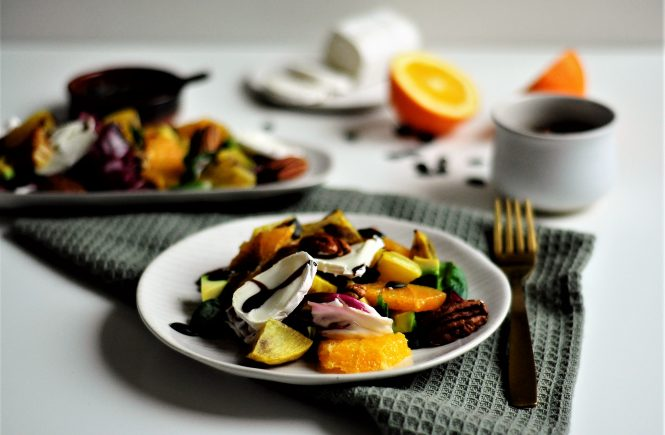
\includegraphics[scale=.6]{pics/Wintersalat}
	\caption{Ein köstlicher Wintersalat}
	\label{fig:Wintersalat}
\end{figure}
\newpage
\subsection{Gegrillter Butternusskürbis-Salat}
Kürbisse eignen sich hervorragend zum Grillen. Als Beilage zum zu gegrillten 
Fisch, Rind und Schwein eignet dieser Salat aus gegrillten Butternusskürbis 
super.

\paragraph{Für den Salat}

\begin{itemize}[noitemsep]
	\item 1 Butternusskürbis (ca. 800g)
	\item 6 EL Olivenöl
	\item 1 Dose (425 g) Kichererbsen
	\item 120 g Blattspinat
	\item 12 Kirschtomaten
	\item 3 Lauchzwiebeln
	\item 1 kleine Salatgurke (ca. 250 g)
	\item 50 g Haselnusskerne
	\item 3 EL Essig (bei mir Altmeister von Hengstenberg)
\end{itemize}

\begin{figure}[htbp]
	\centering
	\includegraphics[scale=.35]{pics/Kürbis1}
	\caption{Gegrillter Butternusskürbis-Salat}
	\label{fig:Kürbis1}
\end{figure}

\paragraph{Zubereitung}

Die Holzspieße in Wasser einweichen. Den Kürbis putzen, längs halbieren und 
das Kerngehäuse entfernen. Das Fruchtfleisch in walnussgroße Stücke 
schneiden
und in reichlich kochendem Salzwasser ca. 6 Minuten kochen. Die gekochten 
Kürbisstücke abgießen und unter fließendem kalten Wasser abkühlen. Die 
Kürbisstücke gut abtropfen lassen und mit 3 EL Olivenöl in eine Schüssel 
mischen. Danach mit Salz und Pfeffer würzen.

Kürbis auf Holzspieße stecken. In einer Grillschale auf dem heißen Grill 6–8 
Minuten unter Wenden grillen. Holzspieße vom Grill nehmen. Kürbisstücke von 
den 
Spießen in eine Schüssel streifen.

Kichererbsen in einem Sieb gut abtropfen lassen. Blattspinat putzen, waschen 
und trocken schleudern. Tomaten waschen und halbieren. Lauchzwiebeln 
waschen,
trocken schütteln und in Ringe schneiden. Gurke putzen, waschen und in 
Würfel schneiden.

Kichererbsen, Spinat, Tomaten, Lauchzwiebeln, Gurke, Haselnüsse, Essig und 
restliches Öl zum Kürbis geben und vorsichtig untermischen. Mit Salz und 
Pfeffer
abschmecken und anrichten, siehe \vref{fig:Kürbis1}.

\section{Weiter geht es mit den Beilagensalaten}

\subsection{Coleslaw}\label{Coleslaw}

Coleslaw ist ein amerikanischer Krautsalat, der hauptsächlich aus fein 
geschnittenem Weißkohl und Möhren besteht. Was diesen Salat besonders 
macht, ist das cremige Dressing,

Der Coleslaw wird oft als Beilage zu BBQ-Gerichten, Sandwiches oder Burgern 
serviert und ist bekannt für seine erfrischende und gleichzeitig reichhaltige 
Textur. Die Kombination aus knackigem Gemüse und dem cremigen Dressing 
macht ihn zu einem beliebten Gericht bei vielen Gelegenheiten.

\paragraph{Für den Coleslaw}

\begin{itemize}[noitemsep]
	\item 1 Weißkohl (ca. 1,4 kg)
	\item 1 Karotte
	\item 1 Zwiebel, klein
	\item 200g Mayonnaise
	\item 80 g Sahne
	\item 2 EL Weinessig
	\item 4 EL Zucker
	\item 1 TL Selleriesamen
	\item Himalaya-Salz
	\item Schwarzer Pfeffer
\end{itemize}

\paragraph{Zubereitung}

Der Weißkohl wird halbiert, der Strunk entfernt und der Kohl feine Streifen 
geschnitten. Zusammen mit der fein geraspelten Karotte und der fein 
geschnittenen Zwiebel wird der Weißkohl vermischt.

Für die Sauce werden die Mayonnaise, Sahne, Weinessig, Zitronensaft, Zucker 
und Selleriesamen vermischt und mit Salz und Pfeffer abgeschmeckt. Die 
Selleriesamen sollten zuvor im Mörser zerstoßen werden, damit sich das Aroma 
besser entfalten kann. Die fertige Sauce über den Coleslaw geben und gut 
einmassieren. Das ganze über Nach im Kühlschrank durchziehen lassen. Vor 
dem Servieren nachmals gut durchrühren, siehe \vref{fig:Coleslaw}.

\begin{figure}[htbp]
	\centering
	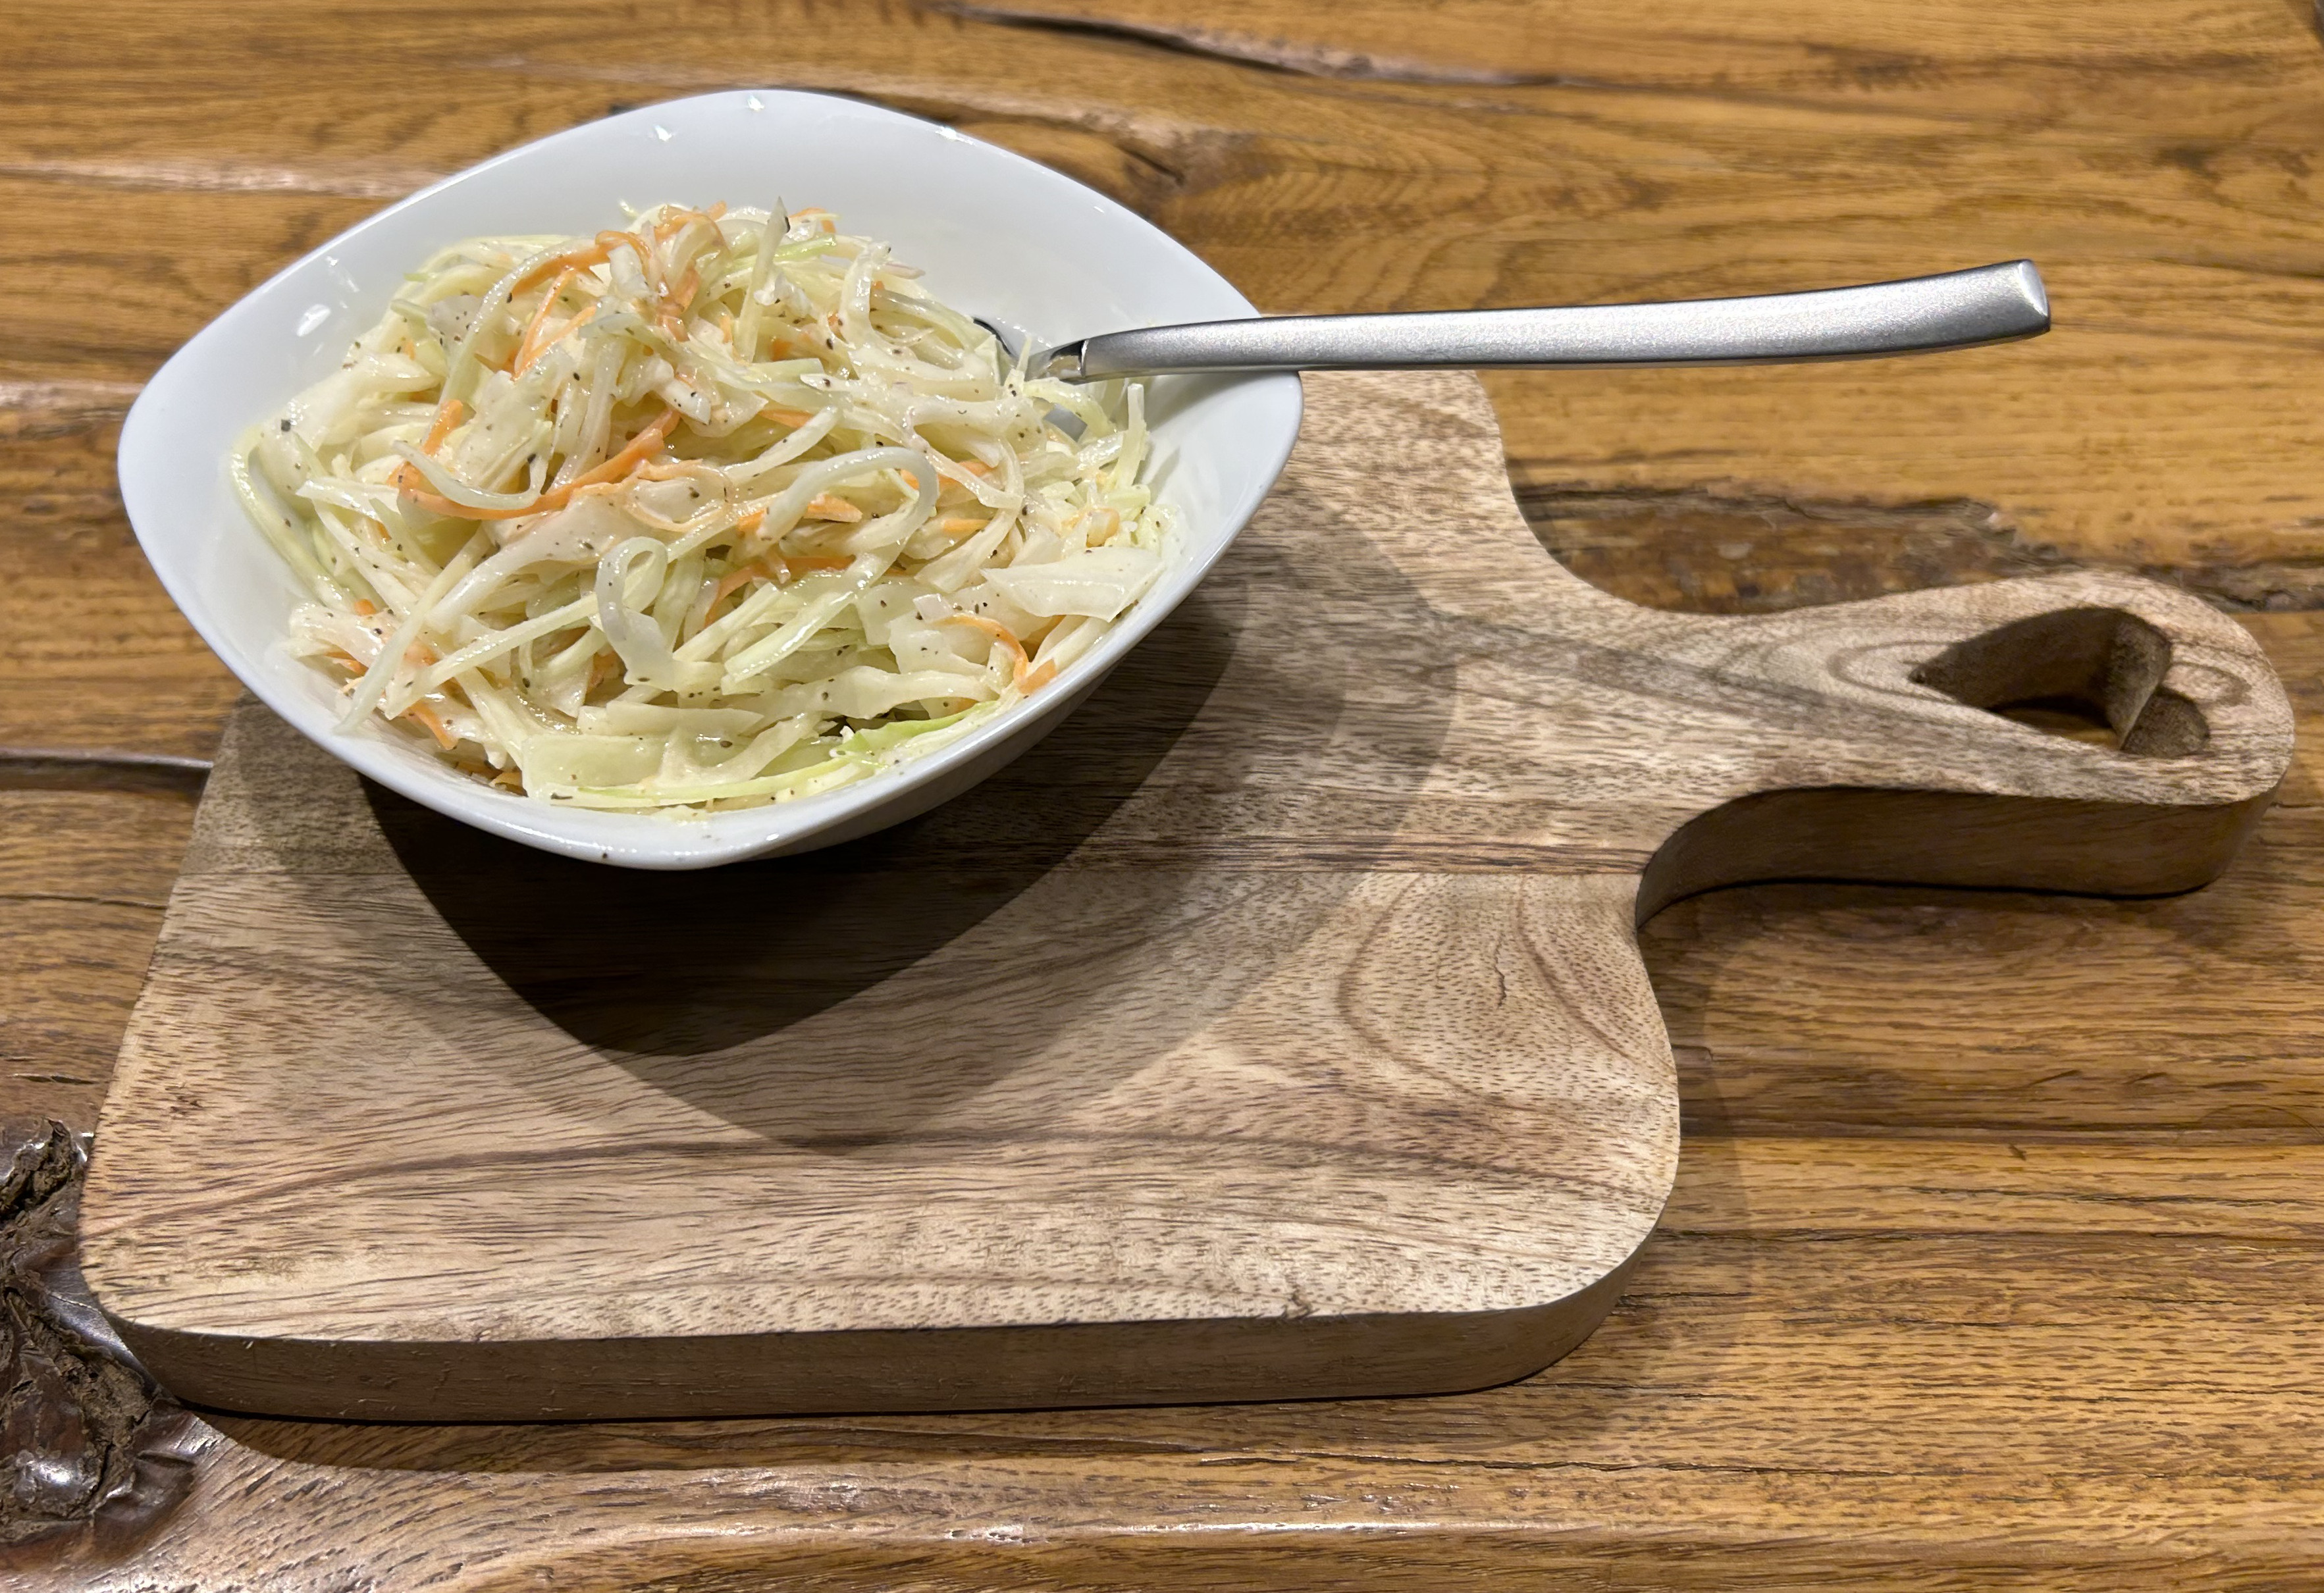
\includegraphics[scale=.4]{pics/Coleslaw}
	\caption{Amerikanischer Krautsalat, sehr gut passend zu BBQ}
	\label{fig:Coleslaw}
\end{figure}

\subsection{Feldsalat mit Mozzarella und Tomatendressing}

\paragraph{Für den Salat}

\begin{itemize}[noitemsep]
	\item 1 L Tomatensaft
	\item 1 Zwiebel
	\item 1 Knoblauchzehe
	\item 2 EL Zucker
	\item 150 ml Balsamico oder Apfelessig
	\item 4 Kugeln Mozzarella
	\item 500g Feldsalat
	\item 200g Bacon
	\item 2 Tomaten
\end{itemize}

\paragraph{Zubereitung}

Die Zwiebel und  Knoblauchzehe fein schneiden. In Olivenöl anschwitzen.
Den Zucker zugeben und leicht karamellisieren. Mit dem Essig ablöschen und 
reduzieren.
Tomatensaft hinzugeben,  auf 1/3 der Menge reduzieren und von der Flamme 
nehmen. 
Die Tomaten entkernen und in Würfel schneiden

Die Mozzarellakugel in der Mitte des Tellers platzieren Tomatendressing leicht 
aufwärmen und rund
um die Mozzarellakugel verteilen.  Den Feldsalat auf dem Dressing drapieren 
die Tomaten darauf verteilen 
und alles mit Olivenöl beträufeln. Die angebratenen Baconscheiben halbieren 
und auf den Feldsalat legen. 
Die Mozzarellakugel kreuzförmig einschneiden und mit dem angewärmten 
Tomatendressing übergießen. 
Den Salat servieren.

\subsection{Eisbergsalat mit Champignons und Tomatendressing}

\paragraph{Für den Salat}

\begin{itemize}[noitemsep]
	\item 1 Eisbergsalat
	\item 1 Schale Champignons
	\item Olivenöl
	\item 1 Zehe Knoblauch
\end{itemize}

Zutaten für das Dressing:
\begin{itemize}[noitemsep]
	\item 1l Tomatensaft
	\item 1 kleine Zwiebel
	\item 1 Knoblauchzehe
	\item 150 Essig Balsamico oder Apfelessig
	\item 2 EL Zucker
	\item 1 Tomate
\end{itemize}

\paragraph{Zubereitung}

Die Zwiebel und  Knoblauchzehe fein schneiden. In Olivenöl anschschwitzen.
Den Zucker zugeben und leicht karamellisieren. Mit dem Essig ablöschen und 
reduzieren.
Tomatensaft hinzugeben,  auf 1/3 der Menge reduzieren und von der Flamme 
nehmen. 
Die Tomaten entkernen und in Würfel schneiden.

Die Champignons in Scheiben,  die Tomate entkernen und in Würfel schneiden. 
Die Champignons mit dem Knoblauch in 
Olivenöl anbraten. Dressing auf den Salattellern verteilen. Den Eisbergsalat, 
trocknen und auf dem Dressing verteilen. Den 
Salat mit den Champignons und Tomatenwürfeln anrichten und servieren.
